% !TEX encoding = UTF-8 Unicode
% !TEX root = ../rapport.tex

\chapter{Algorithme d'exclusion mutuelle de Naimï-Trehel}\label{naimi-trehel}


\section{Description}
L'algorithme de Naimi-Trehel \cite{naimi1996} est basé sur le fait de conserver deux structures de données distribuées et un jeton. Le jeton est présent sur un des sites à la fois et matérialise la permission d'entrer en section critique. Les structures de données distribuées sont un arbre logique dynamique et une file d'attente.

La file d'attente stocke les sites qui ont demandé à entrer en section critique. La file d'attente étant distribuée, chaque site stocke uniquement son suivant (s'il y en a un) dans la file d'attente. La tête de la file est le site actuellement en section critique et la queue de la file est le dernier site à avoir demandé à y entrer. Quand un site demande à entrer en section critique, il est ajouté à la fin de la file. Quand un site quitte la section critique, il envoie le jeton à son suivant dans la file (s'il y en a un).

La seconde structure de données est l'arbre logique dynamique. Cet arbre a pour but d'indiquer aux sites lequel d'entre eux est le dernier dans la file d'attente. La structure étant distribuée, chaque site stocke uniquement son père dans l'arbre. Lorsqu'un site veut entrer en section critique, il transmet la requête à son père qui (s'il n'est pas racine) transmet la requête à son père jusqu'à ce que la requête atteigne la racine de l'arbre. Le site racine dans l'arbre étant également le dernier dans la file d'attente, il fixe son suivant au site qui a émis la requête. Puis tous les sites qui ont transmis la requête fixent leur père au site qui a émis la requête (désormais le dernier dans la file d'attente).


\section{Exemple}

\tikzstyle{vertex}=[circle,fill=black!25,minimum size=20pt,inner sep=0pt]
\tikzstyle{edge} = [draw,thick,-]
\tikzstyle{tree edge} = [draw, thick,->,red!75]
\tikzstyle{queue edge} = [draw,thick,->,green!50]

Dans cet exemple, initialement, le nœud $a$ possède le jeton (figure \ref{naimi-trehel-exemple1}).
\begin{figure}[H]
\label{naimi-trehel-exemple1}
\begin{minipage}[b]{0.32\linewidth}
\centering
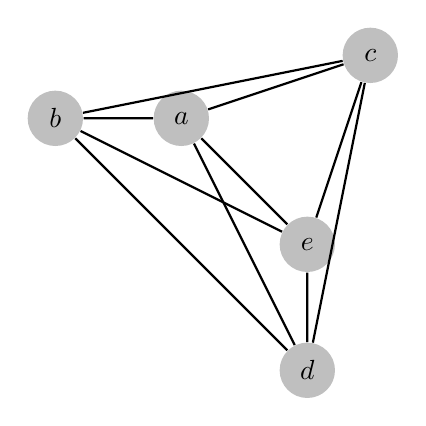
\begin{tikzpicture}[scale=0.8,auto,swap]
		\node[vertex] (a) at (2,4) {$a$};
		\node[vertex] (b) at (0,4) {$b$};
		\node[vertex] (c) at (5,5) {$c$};
		\node[vertex] (d) at (4,0) {$d$};
		\node[vertex] (e) at (4,2) {$e$};
    		% First we draw the vertices
		\draw (a) (b) (c) (d) (e);
   		 % Connect vertices with edges
   		\foreach \source/ \dest in {a/b, a/c, a/d, a/e, b/c, b/d, b/e, c/d, c/e, d/e}
        		\path[edge] (\source) -- (\dest);
\end{tikzpicture}
\caption{Réseau physique}
\end{minipage} 
\hspace{0.1cm}
\begin{minipage}[b]{0.32\linewidth}
\centering
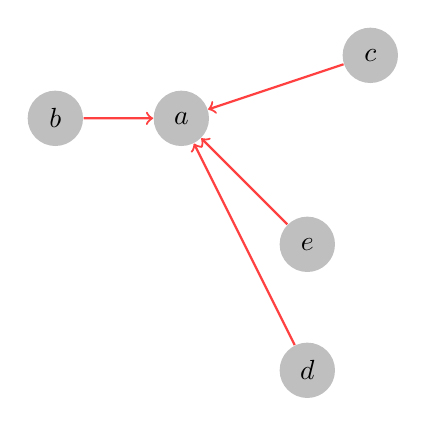
\begin{tikzpicture}[scale=0.8,auto,swap]
	\node[vertex] (a) at (2,4) {$a$};
		\node[vertex] (b) at (0,4) {$b$};
		\node[vertex] (c) at (5,5) {$c$};
		\node[vertex] (d) at (4,0) {$d$};
		\node[vertex] (e) at (4,2) {$e$};
    		% First we draw the vertices
		\draw (a) (b) (c) (d) (e);
   		 % Connect vertices with edges
   		 \foreach \source/ \dest in {b/a, c/a, d/a, e/a}
		 \path[tree edge] (\source) to (\dest);
\end{tikzpicture}
\caption{Arbre logique}
\end{minipage} 
\hspace{0.1cm}
\begin{minipage}[b]{0.32\linewidth}
\centering
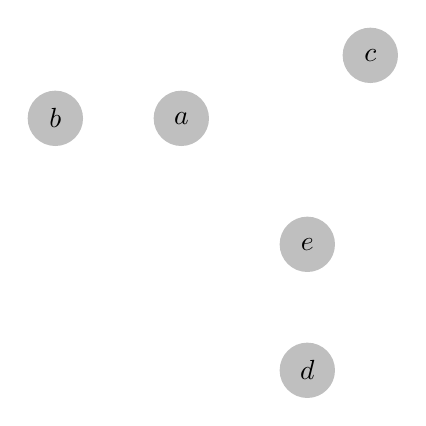
\begin{tikzpicture}[scale=0.8,auto,swap]
		\node[vertex] (a) at (2,4) {$a$};
		\node[vertex] (b) at (0,4) {$b$};
		\node[vertex] (c) at (5,5) {$c$};
		\node[vertex] (d) at (4,0) {$d$};
		\node[vertex] (e) at (4,2) {$e$};
    		% First we draw the vertices
		\draw (a) (b) (c) (d) (e);
\end{tikzpicture}
\caption{File d'attente}
\end{minipage}
\end{figure}

Puis le nœud $b$ fait une requête pour obtenir la section critique.


\section{Propriétés}

